\chapter{A módszer kiértékelése}
\label{ch:eval}

A modern szemantikus reprezentációs algoritmusok célja, olyan univerzális és általános modellek előállítása, amelyek bármely rendszerben képesek igazodni az adott kihívásokhoz és megfelelő pontossággal teljesíteni az eléjük tűzött feladatokat.

A nyelvi modellek teljesítményének mérése nem triviális feladat. Bár a publikációk során a szerzők többnyire saját módszerrel mérnek, vannak már meglévő komplex kiértékelési keretrendszerek – például SentEval \cite{senteval}, GLUE \cite{glue} – és az igény is egyre nagyobb ezekre. A teljesítmény mérésére szolgáló rendszerek segítségével egységes képet kaphatunk a módszerünk pontosságáról, illetve a csalás lehetősége is korlátozott. A kiértékelés közben a reprezentációs modelleknek olyan feladatok sorozatát kell megoldaniuk, mint a vélemény-polaritás, bináris érzelmi analízis, következtetés vizsgálat, szemantikus hasonlóság.

Mivel a munkám során tanított modellek mindegyike magyar nyelvű, így nem használhattam ezen megoldásokat. Szükségem volt egy saját kiértékelési feladat implementálására.

\section{Árukereső kommentek bináris érzelmi analízise}

Az általam létrehozott modellek pontosságának mérésére használt feladatnak több szempont szerint is meg kellett felelni. Jó kiértékelési feladat az, amelyik kellőképpen "nehéz", így a modellek közti teljesítménybeli különbségek jól interpretálhatóak. Továbbá a feladathoz tartozó adathalmaznak elegendő elemet kell tartalmaznia ahhoz, hogy a feladat elkerülje a túltanulás problémáját és hiteles kimenetet kapjunk végeredményül. Az \textit{arukereso}-nek nevezett adathalmaz bináris osztályozása a vélemények érzelmi tartalma alapján megfelelő kihívásnak minősült ahhoz, hogy az általam tanított modellek pontosságát meg tudjam határozni.

A mérés során az annotált tanítóhalmaz elemeit – azaz pozitív vagy negatív osztályba tartozó értékeléseket – a meglévő modellek segítségével vektortérbe képeztem. Majd az így kapott vektor-címke párokkal tanítottam különféle osztályozó algoritmusokat. Ezen algoritmusok teszthalmazon történő kiértékelésének kimenete adta meg az adott szemantikus modell pontosságát.

Szükségem volt egy olyan viszonyítási alapra, amely a már létező magyar nyelvű módszerek teljesítményét szimbolizálja. Erre a célra az értékelések szavait az előre betanított \textit{oscar} és \textit{oscar\_sm} Word2Vec modellekkel leképezve, majd átlagolva megkaptam a véleményeket reprezentáló 300 hosszú vektorokat. Mivel az értékelések változó méretűek, továbbá legalább 10 token-ből állnak, a BiLSTM modellek esetén csak az első 201 token került a bemenetre a vektorok generálása során. A túl rövid paragrafusokat a tanításhoz hasonlóan \textit{padding}-eltem.

Egy bináris osztályozási feladat teljesítménye többféle metrika szerint is mérhető. Ezek közül a legnépszerűbb a klasszifikációs \textbf{pontosság} (\textit{accuracy}), amely a helyesen prediktált elemek számának és az összes elem számának hányadosa. A \textbf{tévesztési mátrix} (\textit{confusion matrix}) leírja és vizualizálja modellünk teljesítményét az igaz pozitívként, igaz negatívként, hamis pozitívként és hamis negatívként prediktált elemek számának segítségével. A \textbf{vevő működési karakterisztika} (\textit{receiver operating characteristic} - ROC) görbe az igaz pozitív és a hamis pozitív arányok közötti kapcsolatot szemlélteti. Egy véletlenszerű modell görbéje a főátlón helyezkedik el, ahol a függőleges tengelyen az igaz pozitív, a vízszintes tengelyen a hamis pozitív arányok szerepelnek. Minél nagyobb a görbe alatti terület, annál jobb a modellünk performanciája.

\begin{table}[H]
	\centering
	\begin{tabular}{ | c | r | r | r | r | r | r | r |}
		\hline
		\multirow{2}{*}{\textbf{Modell / Osztályozó}} & \multirow{2}{*}{\textbf{Linear SVM}} & \multirow{2}{*}{\textbf{XGBoost}} & \multirow{2}{*}{\textbf{Random Forest}} \\
		& & & \\
		\hline \hline		
		\textbf{w2v\_sm} & 85,45\% & 82,18\% & 83,64\% \\
		\hline
		\textbf{w2v\_sm\_norm} & 85,57\% & 82,71\% & \textbf{84,18\%} \\
		\hline
		\textbf{w2v\_lg} & 85,28\% & 82,87\% & 83,77\% \\
		\hline
		\textbf{w2v\_lg\_norm} & 85,59\% & 83,15\% & 83,85\% \\
		\hline  
		\textbf{lstm\_1024} & 81,53\% & 80,82\% & 80,84\% \\
		\hline  
		\textbf{lstm\_1024\_norm} & 85,37\% & 83,48\% & 83,41\% \\
		\hline
		\textbf{lstm\_4096\_norm} & \textbf{87.16\%} & \textbf{83,71\%} & 83,90\% \\
		\hline
	\end{tabular}
	\caption[A modellek pontossága]{A modellek klasszifikációs pontossága az arukereso adathalmazon. A w2v\_sm az oscar\_sm, a w2v\_lg az oscar halmazon tanított modelleket, a norm posztfix a normált bemenetet jelöli. A számok a modellek nevében a reprezentációs vektor méretére utalnak.}
	\label{tab:evaluation}
\end{table}

Az \ref{tab:evaluation}-es táblázat az arukereso adathalmazon mért klasszifikációs pontosságokat foglalja össze. A kiértékeléshez használt osztályozó algoritmusok a Linear SVM, XGBoost és Random Forest. A \textit{w2v\_sm} Word2vec modellt az \textit{oscar\_sm} halmazon, a \textit{w2v\_lg}-t az \textit{oscar} halmazon tanítottam. Az \textit{lstm} prefixű modellek a bemutatott módszerrel előállított nyelvi modellek.

A mért eredmények azt mutatják, hogy az általam ismertetett módszer esetén a bemeneti rétegnek átadott \textit{w2v\_sm} és a jelentősen nagyobb szótárral rendelkező \textit{w2v\_lg} teljesítménye közötti különbség elenyésző. Továbbá a normált bemenettel tanított modellek használata közben az algoritmusok nagyobb százalékban osztályoznak megfelelően. A feladatot legnagyobb pontossági értékkel abszolváló modell az \textit{lstm\_4096\_norm}, amely alkalmazása során a helyesen klasszifikált elemek aránya 87,16\% volt.

\begin{figure}[H]
	\centering
	\subfigure[lstm\_4096\_norm]{
		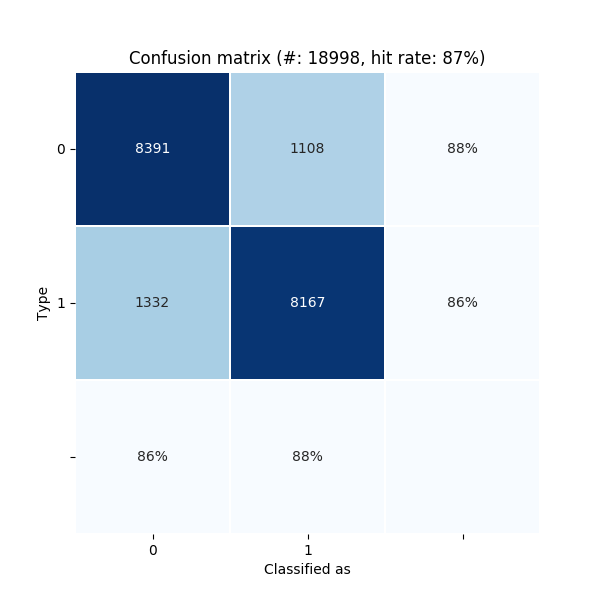
\includegraphics[width=0.6\linewidth]{matrix-4096}}
	\subfigure[w2v\_lg\_norm]{
		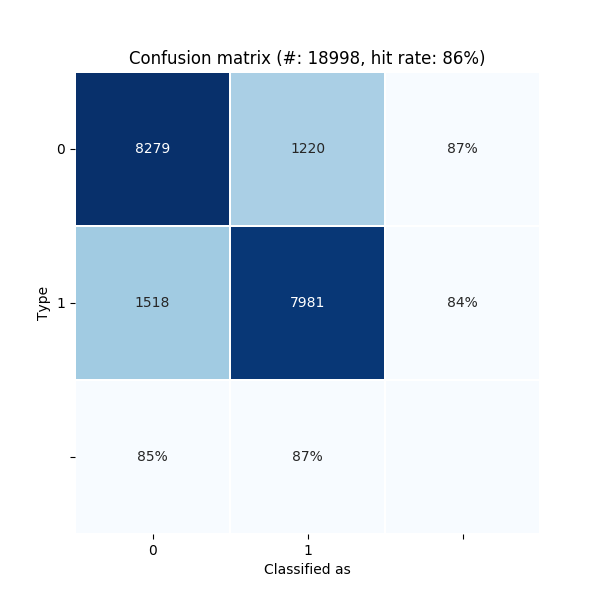
\includegraphics[width=0.6\linewidth]{matrix-w2v}}
	\caption{A legjobban teljesítő LSTM és Word2Vec alapú modellek tévesztési mátrixa}
	\label{fig:matrix}
\end{figure}

Az \ref{fig:matrix}-es ábra a legpontosabb általam bemutatott és Word2Vec alapú modell tévesztési mátrixát ábrázolja a Linear SVM oszályozó algoritmusra. Az \textit{lstm\_4096\_norm} segítségével az osztályozó 298 esetben helyes döntést hozott, míg a Word2Vec vektorok alkalmazása során helytelenül választott. Az igaz pozitív, igaz negatív, hamis pozitív, hamis negatív csoportok a két esetben relatíve kiegyensúlyozottak.

\begin{figure}[H]
	\centering
	\subfigure[lstm\_4096\_norm]{
		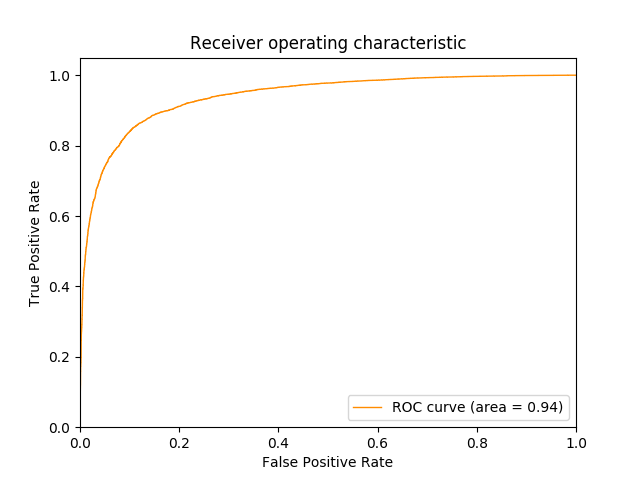
\includegraphics[width=0.6\linewidth]{roc-4096}}
	\subfigure[w2v\_lg\_norm]{
		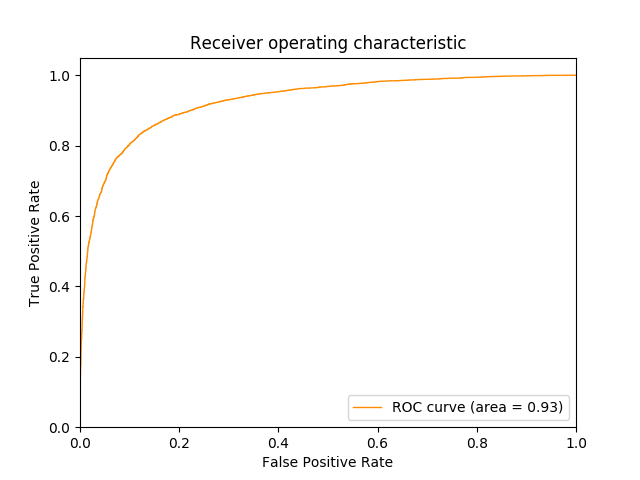
\includegraphics[width=0.6\linewidth]{roc-w2v}}
	\caption{A legjobban teljesítő LSTM és Word2Vec alapú modellek ROC görbéje}
	\label{fig:roc}
\end{figure}

Az \ref{fig:roc}-es ábra a fent található tévesztési mátrixokhoz tartozó ROC görbéket illusztrálja. Az \textit{lstm\_4096\_norm} modellre vonatkozó függvény görbe alatti területe nagyobb, mint a Word2Vec modell esetén, amely szerint az LSTM alapú reprezentációs módszer segítségével a Linear SVM algoritmus pontosabb osztályozásra képes.

KONKLÚZIÓ


BEFEJEZÉS


%befejezés:
%saját halmaz - nem túl kiterjedt, tehát nem a nyelvi modell egészét méri de adott feladatra jó - cite

% kód cite

%más módszereket is ki lehet vele mérni, publikusan elérhető adathalmaz







